\documentclass[11pt, a4paper]{article}

\usepackage[margin=2.5cm]{geometry}
\usepackage{amsmath, amssymb, amsthm}
\usepackage{bm}
\usepackage{xcolor}
\usepackage{booktabs}
\usepackage{array}
\usepackage{tikz}
\usetikzlibrary{arrows.meta, positioning, shapes.geometric,
                fit, backgrounds, calc, decorations.pathreplacing}
\usepackage{algorithm}
\usepackage{algpseudocode}
\usepackage{hyperref}
\usepackage{enumitem}
\usepackage{mdframed}
\usepackage{caption}

% ── Colours ───────────────────────────────────────────────────────────────────
\definecolor{aifblue}{RGB}{30, 90, 180}
\definecolor{aifgreen}{RGB}{0, 140, 80}
\definecolor{aifgray}{RGB}{90, 90, 90}
\definecolor{aifred}{RGB}{180, 40, 40}
\definecolor{aifpurple}{RGB}{120, 40, 160}
\definecolor{aiforange}{RGB}{200, 110, 0}
\definecolor{boxbg}{RGB}{240, 246, 255}
\definecolor{warningbg}{RGB}{255, 248, 230}
\definecolor{greenbg}{RGB}{235, 250, 238}

\newmdenv[backgroundcolor=boxbg, linecolor=aifblue,
          linewidth=1.5pt, roundcorner=4pt,
          innertopmargin=8pt, innerbottommargin=8pt]{keybox}
\newmdenv[backgroundcolor=warningbg, linecolor=aiforange,
          linewidth=1.5pt, roundcorner=4pt,
          innertopmargin=8pt, innerbottommargin=8pt]{notebox}
\newmdenv[backgroundcolor=greenbg, linecolor=aifgreen,
          linewidth=1.5pt, roundcorner=4pt,
          innertopmargin=8pt, innerbottommargin=8pt]{resultbox}

% ── Macros ─────────────────────────────────────────────────────────────────────
\newcommand{\vect}[1]{\bm{#1}}
\newcommand{\mat}[1]{\mathbf{#1}}
\newcommand{\FE}{\mathcal{F}}
\newcommand{\norm}[1]{\left\|#1\right\|}
\newcommand{\Pip}{\mat{\Pi}_p}
\newcommand{\Pisl}{\mat{\Pi}_s^{\text{low}}}
\newcommand{\Pish}{\Pi_s^{\text{high}}}
\newcommand{\epsp}{\vect{\varepsilon}_p}
\newcommand{\epss}{\vect{\varepsilon}_s}

\title{%
  \textbf{\Large Hierarchical Active Inference for Trajectory Tracking}\\[4pt]
  \large A Two-Tier Model: Continuous Low-Level Agent
  $+$ Discrete High-Level Agent\\[2pt]
  \normalsize with Efference Copy, Precision Modulation,
  and Cross-Modal Surprise
}
\author{}
\date{}

\begin{document}
\maketitle\thispagestyle{empty}
\tableofcontents\newpage

% ══════════════════════════════════════════════════════════════════════════════
\section{Motivation and Overview}

The single-level continuous agent (documented separately) successfully tracks
a 3-D trajectory under gravity but has no mechanism to respond to unexpected
events. The hierarchical extension adds a \textbf{discrete high-level agent}
that monitors for surprising cross-modal stimuli and — through
\emph{precision modulation} — transiently perturbs the low-level controller.

The model is designed to reproduce a specific experimental signature:

\begin{resultbox}
\textbf{Target phenomenology (from experiments).}
\begin{itemize}[noitemsep]
  \item Sudden, task-irrelevant stimuli produce \textbf{triphasic kinematic
        perturbations} (decrease–increase–decrease in acceleration) aligned
        with the dominant force axis.
  \item Perturbations are \textbf{larger during movement} than during
        stationary holding.
  \item Electrocortical responses (vertex potentials) are
        \textbf{smaller during movement} — an anti-correlation.
\end{itemize}
One mechanism must account for both signatures simultaneously.
\end{resultbox}

% ══════════════════════════════════════════════════════════════════════════════
\section{Architecture}

The model has two tiers that exchange information every timestep.

\subsection{State and action spaces (low level)}
Unchanged from the single-agent model:
\begin{equation}
  \vect{x} = [p_1, p_2, p_3, v_1, v_2, v_3]^\top \in \mathbb{R}^6,
  \qquad
  \vect{a} = [u_1, u_2]^\top \in \mathbb{R}^2, \quad u_3 \equiv 0.
\end{equation}

\subsection{State space (high level)}
The discrete agent maintains a categorical belief over three states:
\begin{equation}
  s \in \{\underbrace{\text{TRACK}}_{0},\;
          \underbrace{\text{SURPRISED}}_{1},\;
          \underbrace{\text{RECOVER}}_{2}\},
  \qquad
  \vect{s}_t \in \Delta^2 \;\;(\text{probability simplex}).
\end{equation}

\subsection{Coupling signals}
\begin{center}
\renewcommand{\arraystretch}{1.4}
\begin{tabular}{lll}
\toprule
\textbf{Signal} & \textbf{Direction} & \textbf{Definition} \\
\midrule
Efference copy & low $\to$ high &
  $e(t) = \norm{\vect{a}(t)}$,\quad
  $\bar{e}(t) = e(t)/a_{\max} \in [0,1]$ \\
Precision scale & high $\to$ low &
  $\Pisl(t) = \sigma_{\text{low}}(\gamma(t))\,\mat{\Pi}_s^{\text{base}}$ \\
\bottomrule
\end{tabular}
\end{center}

% ══════════════════════════════════════════════════════════════════════════════
\section{High-Level Discrete Agent}
\label{sec:high}

\subsection{Observation model}
The high-level agent receives a binary cross-modal observation
$o_t \in \{0\text{ (no stim)},\, 1\text{ (stim)}\}$.
The likelihood matrix $\mat{A} \in [0,1]^{3\times 2}$ encodes that
\textsc{Surprised} is the only state consistent with stimulus presence:
\begin{equation}
  \mat{A} =
  \begin{pmatrix}
    0.95 & 0.05 \\
    0.05 & 0.95 \\
    0.90 & 0.10
  \end{pmatrix},
  \quad
  A_{s,o} = p(o_t = o \mid s_t = s).
\end{equation}

\subsection{Transition model — efference modulation}
The transition matrix $\mat{B}(\bar{e})$ is modulated by the normalised
efference copy $\bar{e}(t) \in [0,1]$:

\begin{equation}
  p(\text{TRACK} \to \text{SURPRISED}) = p_0 + \alpha_B\,\bar{e}, \qquad
  p(\text{SURP} \to \text{RECOVER})   = q_0 + \alpha_B\,\bar{e}, \qquad
  p(\text{REC}  \to \text{TRACK})     = r_0 + \alpha_B\,\bar{e}.
\end{equation}

\begin{keybox}
\textbf{Interpretation.}
High motor activity (large $\bar{e}$) makes the system easier to
destabilise (\textsc{Track}$\to$\textsc{Surprised} more likely) and
accelerates recovery (\textsc{Surprised}$\to$\textsc{Recover}$\to$\textsc{Track}
faster). This is the mechanism by which the \emph{same} stimulus produces a
larger kinematic effect during movement.
\end{keybox}

\subsection{Belief update — softmax over log-likelihoods}
Following standard discrete AIF, the belief is updated in two steps:

\paragraph{Step 1 — Prior prediction.}
\begin{equation}
  \vect{s}_{\text{prior}} = \mat{B}(\bar{e})\,\vect{s}_{t-1},
  \qquad \vect{s}_{\text{prior}} \in \Delta^2.
\end{equation}

\paragraph{Step 2 — Bayesian update (posterior).}
\begin{equation}
  \tilde{s}_t(s) \propto A_{s,\,o_t} \cdot s_{\text{prior}}(s),
  \qquad
  \vect{s}_t = \frac{\tilde{\vect{s}}_t}{\norm{\tilde{\vect{s}}_t}_1}.
\end{equation}
This is equivalent to softmax over log-likelihoods:
\begin{equation}
  \ln \vect{s}_t = \ln \vect{s}_{\text{prior}}
                 + \ln \mat{A}_{:,\,o_t} + \text{const}.
\end{equation}

\subsection{Surprise and high-level free energy}
\begin{align}
  p(o_t) &= \sum_s A_{s,o_t}\,s_{\text{prior}}(s) \quad
            (\text{marginal likelihood}),\\[4pt]
  \xi_t   &= -\ln p(o_t) \quad (\text{surprise}),\\[4pt]
  \FE_{\text{high},t}
          &= \underbrace{D_{\mathrm{KL}}[\vect{s}_t \| \vect{s}_{\text{prior}}]}_{\text{belief update cost}}
           + \underbrace{\xi_t}_{\text{surprise}}.
  \label{eq:fe_high}
\end{align}
Both $\xi_t$ and $\FE_{\text{high},t}$ are stored as
\textbf{candidate proxies for the vertex potential}
(see Sec.~\ref{sec:vp}).

% ══════════════════════════════════════════════════════════════════════════════
\section{Precision Coupling}
\label{sec:coupling}

\subsection{Surprise pulse $\gamma(t)$}
The high-level surprise $\xi_t$ drives a leaky-integrator pulse:
\begin{equation}
  \dot{\gamma} = -\frac{\gamma}{\tau_\gamma} + \lambda_\gamma\,\xi_t,
  \qquad \gamma(0) = 0, \quad \gamma \geq 0.
  \label{eq:gamma}
\end{equation}
The pulse rises sharply at stimulus onset and decays exponentially
with time constant $\tau_\gamma$.

\subsection{Low-level precision modulation}
\begin{equation}
  \boxed{
  \Pisl(t) = \frac{1}{1+\gamma(t)}\;\mat{\Pi}_s^{\text{base}},
  }
  \label{eq:pisl}
\end{equation}
where $\mat{\Pi}_s^{\text{base}}$ is the baseline 6$\times$6 precision matrix
(z-entries zero, as before). When $\gamma \uparrow$, low-level sensory
precision drops: the agent \emph{loosens its grip} on the trajectory,
generating the kinematic perturbation.

\subsection{High-level precision modulation}
\begin{equation}
  \boxed{
  \Pish(t) = \frac{\Pi_s^{\text{high,base}}\,(1+\gamma(t))}{1 + \alpha_{\text{eff}}\,\bar{e}(t)},
  }
  \label{eq:pish}
\end{equation}
where $\alpha_{\text{eff}} > 0$ controls efference suppression.
When $\bar{e}(t)$ is large (active movement), $\Pish$ is suppressed at
baseline — representing predictive motor suppression.

\begin{notebox}
\textbf{Independence of the two precisions.}
$\Pisl$ and $\Pish$ are \emph{not} coupled by a conservation law.
They happen to move in opposite directions at stimulus onset because
both are functions of $\gamma(t)$, but through independent pathways.
\end{notebox}

% ══════════════════════════════════════════════════════════════════════════════
\section{Low-Level Continuous Agent}
\label{sec:low}

The low-level equations are identical to the single-agent version
except that $\Pisl$ is now time-varying.

\subsection{Belief update}
\begin{equation}
  \dot{\vect{\mu}} = \vect{f}_{\text{model}}(\vect{\mu}, \vect{a})
    + \kappa_\mu\bigl(\Pisl(t)\,\epss - \Pip\,\epsp\bigr).
  \label{eq:mu_dot}
\end{equation}

\subsection{Precision-modulated action}
The PD controller is scaled by the low-level precision:
\begin{align}
  u_1 &= \sigma(\gamma)\,m_1\bigl[K_P(p_1^*-\mu_{p_1})
         + K_D(v_1^*-\mu_{v_1})\bigr], \label{eq:u1}\\
  u_2 &= \sigma(\gamma)\,m_2\bigl[K_P(p_2^*-\mu_{p_2})
         + K_D(v_2^*-\mu_{v_2})\bigr] + m_2 g, \label{eq:u2}
\end{align}
where $\sigma(\gamma) = 1/(1+\gamma) \in (0,1]$ is the precision scale.

\begin{keybox}
\textbf{Origin of the triphasic perturbation.}
At stimulus onset $\gamma$ rises sharply, so $\sigma(\gamma) \to 0$:
\begin{enumerate}[noitemsep]
  \item \textbf{Phase 1 (decrease):} PD forces drop — the agent loses grip.
  \item \textbf{Phase 2 (increase):} $\gamma$ begins to decay; position error
        has grown, so forces overshoot as the controller re-engages.
  \item \textbf{Phase 3 (decrease):} Normal convergence to $\vect{x}^*$.
\end{enumerate}
The perturbation is automatically \emph{force-aligned} because it acts through
the force channel, not through a spatial direction vector.
\end{keybox}

\subsection{Low-level free energy}
\begin{equation}
  \FE_{\text{low}} = \tfrac{1}{2}\epsp^\top\Pip\epsp
                   + \tfrac{1}{2}\epss^\top\Pisl(t)\epss.
\end{equation}

% ══════════════════════════════════════════════════════════════════════════════
\section{Vertex Potential Proxies}
\label{sec:vp}

The vertex potential (N100/P300 complex in EEG) reflects neural surprise.
Two candidate proxies are generated by the model:

\begin{center}
\renewcommand{\arraystretch}{1.5}
\begin{tabular}{lll}
\toprule
\textbf{Proxy} & \textbf{Expression} & \textbf{Interpretation} \\
\midrule
$\text{VP}_{\Pi\varepsilon}$ &
  $\Pish(t)\,\norm{\vect{\varepsilon}_s^{\text{high}}(t)}$ &
  Precision-weighted prediction error \\
$\text{VP}_{\FE}$ &
  $\FE_{\text{high},t}$ (Eq.~\ref{eq:fe_high}) &
  Full high-level free energy \\
\bottomrule
\end{tabular}
\end{center}

Both are stored in the simulation output so they can be regressed against
empirical EEG amplitudes to determine which is the better neural correlate.

\paragraph{Predicted anti-correlation.}
During movement $\bar{e}(t)$ is large, suppressing $\Pish$ via the
denominator of Eq.~(\ref{eq:pish}), so both proxies are attenuated at
stimulus onset. The kinematic disruption is large because $\vect{a}$ was large
before the reset. During stationary $\bar{e} \approx 0$, so $\Pish$ is at
its maximum and both proxies are large — but the kinematic disruption is small
because the forces being reset were near zero.

% ══════════════════════════════════════════════════════════════════════════════
\section{Algorithm}

\begin{algorithm}[H]
\caption{Hierarchical AIF — Two-Tier Simulation Loop}
\label{alg:haif}
\begin{algorithmic}[1]
\Require All parameters; likelihood matrix $\mat{A}$; noise arrays
\State \textbf{Init:} $\vect{x}_{\text{real}}, \vect{\mu} \leftarrow \vect{x}_0$;\;
       $\vect{s} \leftarrow [0.95, 0.025, 0.025]$;\;
       $\gamma \leftarrow 0$;\;
       $\vect{a}_{\text{prev}} \leftarrow \vect{0}$
\For{$k = 0,\ldots,N-1$}
  \State $t \leftarrow k\,\Delta t$;\quad
         $\vect{x}^*(t) \leftarrow$ \Call{DesiredState}{$t$}
  \State
  \State \textbf{--- Efference copy ---}
  \State $e \leftarrow \norm{\vect{a}_{\text{prev}}}$;\quad
         $\bar{e} \leftarrow e / a_{\max}$
  \State
  \State \textbf{--- High-level: discrete belief update ---}
  \State $o_t \leftarrow \mathbb{1}[\text{stimulus active at }t]$
  \State $\mat{B} \leftarrow$ \Call{BuildTransitionMatrix}{$\bar{e}$}
  \State $\vect{s}_{\text{prior}} \leftarrow \mat{B}\,\vect{s}$
  \State $p(o_t) \leftarrow \mat{A}_{:,\,o_t}^\top \vect{s}_{\text{prior}}$;\quad
         $\xi \leftarrow -\ln p(o_t)$
  \State $\vect{s} \leftarrow \mat{A}_{:,\,o_t} \odot \vect{s}_{\text{prior}}$;\quad
         normalise $\vect{s}$
  \State $\FE_{\text{high}} \leftarrow
         D_{\mathrm{KL}}[\vect{s}\|\vect{s}_{\text{prior}}] + \xi$
  \State
  \State \textbf{--- Precision pulse update ---}
  \State $\gamma \leftarrow \gamma + \bigl(-\gamma/\tau_\gamma
         + \lambda_\gamma\,\xi\bigr)\,\Delta t$;\quad $\gamma \leftarrow \max(\gamma,0)$
  \State $\sigma \leftarrow 1/(1+\gamma)$
         \hfill\Comment{low-level scale}
  \State $\Pish \leftarrow \Pi_s^{\text{high,base}}\,(1+\gamma)
         \;/\;(1 + \alpha_{\text{eff}}\,\bar{e})$
         \hfill\Comment{high-level precision}
  \State
  \State \textbf{--- Low-level: perception ---}
  \State Build $\Pisl \leftarrow \sigma\,\mat{\Pi}_s^{\text{base}}$
  \State Observe $\vect{y}_{\text{obs}}$ (x-y only, z-entries $\leftarrow \vect{\mu}_z$)
  \State $\epsp \leftarrow \vect{\mu} - \vect{x}^*$;\quad
         $\epss \leftarrow \vect{y}_{\text{obs}} - \vect{\mu}$
  \State $\FE_{\text{low}} \leftarrow \tfrac{1}{2}
         (\epsp^\top\Pip\epsp + \epss^\top\Pisl\epss)$
  \State
  \State \textbf{--- Low-level: action ---}
  \State $u_1 \leftarrow \sigma\,m_1[K_P(\mu_{p_1}^*-\mu_{p_1})
         + K_D(\mu_{v_1}^*-\mu_{v_1})]$
  \State $u_2 \leftarrow \sigma\,m_2[K_P(\mu_{p_2}^*-\mu_{p_2})
         + K_D(\mu_{v_2}^*-\mu_{v_2})] + m_2 g$
  \State Clip $u_1,u_2 \in [-a_{\max}, a_{\max}]$;\quad $u_3\leftarrow 0$;\quad
         $\vect{a}_{\text{prev}} \leftarrow \vect{a}$
  \State
  \State \textbf{--- World update ---}
  \State $\vect{x}_{\text{real}} \leftarrow \vect{x}_{\text{real}}
         + \vect{f}_{\text{proc}}(\vect{x}_{\text{real}},\vect{a},\vect{\omega}_k)\,\Delta t$
  \State
  \State \textbf{--- Belief update ---}
  \State $\vect{\mu} \leftarrow \vect{\mu}
         + \bigl[\vect{f}_{\text{model}}(\vect{\mu},\vect{a})
         + \kappa_\mu(\Pisl\epss - \Pip\epsp)\bigr]\,\Delta t$
  \State
  \State \textbf{--- Vertex potential proxies ---}
  \State $\text{VP}_{\Pi\varepsilon} \leftarrow \Pish\,\norm{\vect{\varepsilon}_{s,xy}}$;\quad
         $\text{VP}_\FE \leftarrow \FE_{\text{high}}$
  \State Store all quantities
\EndFor
\end{algorithmic}
\end{algorithm}

% ══════════════════════════════════════════════════════════════════════════════
\section{System Diagram}

\begin{figure}[ht]
\centering
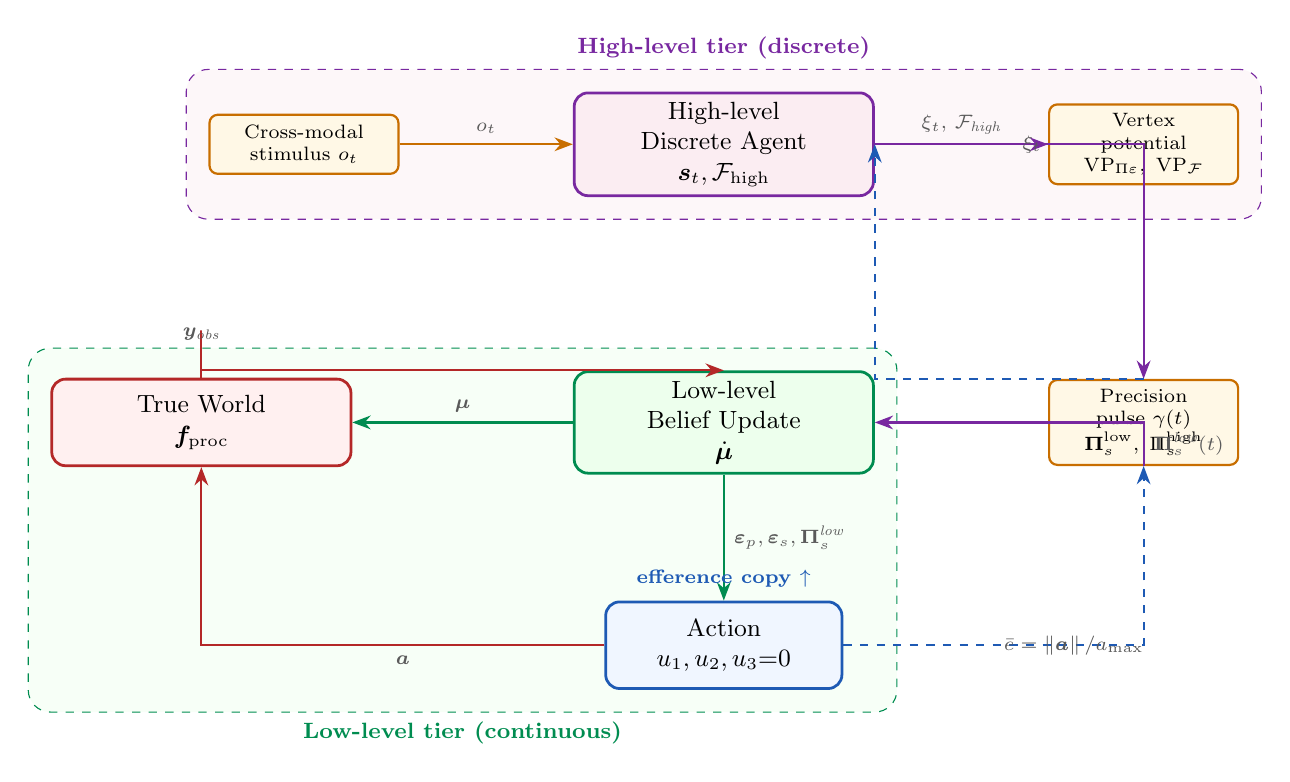
\begin{tikzpicture}[
  node distance=1.4cm and 2.0cm,
  every node/.style={font=\small},
  box/.style={draw, rounded corners=5pt, minimum height=1.1cm,
              minimum width=3.0cm, align=center,
              fill=boxbg, draw=aifblue, line width=1pt},
  hibox/.style={box, fill=purple!7, draw=aifpurple, minimum width=3.8cm},
  lobox/.style={box, fill=green!7,  draw=aifgreen,  minimum width=3.8cm},
  wdbox/.style={box, fill=red!6,    draw=aifred,    minimum width=3.8cm},
  smbox/.style={draw, rounded corners=3pt, minimum height=0.75cm,
                minimum width=2.4cm, align=center, font=\scriptsize,
                fill=warningbg, draw=aiforange, line width=0.8pt},
  arrow/.style={-Stealth, thick},
  lb/.style={font=\scriptsize\itshape, color=aifgray}
]

% ── Nodes ────────────────────────────────────────────────────────────────────
\node[hibox] (hdiscrete)
  {High-level\\Discrete Agent\\$\vect{s}_t, \FE_{\text{high}}$};

\node[smbox, left=2.2cm of hdiscrete] (stim)
  {Cross-modal\\stimulus $o_t$};

\node[lobox, below=2.2cm of hdiscrete] (loperc)
  {Low-level\\Belief Update\\$\dot{\vect{\mu}}$};

\node[wdbox, left=2.8cm of loperc] (world)
  {True World\\$\vect{f}_{\text{proc}}$};

\node[box,   below=1.6cm of loperc] (action)
  {Action\\$u_1, u_2, u_3{=}0$};

\node[smbox, right=2.2cm of hdiscrete] (vp)
  {Vertex\\potential\\$\text{VP}_{\Pi\varepsilon},\;\text{VP}_\FE$};

\node[smbox, right=2.2cm of loperc] (gamma)
  {Precision\\pulse $\gamma(t)$\\$\Pisl,\;\Pish$};

% ── Arrows ────────────────────────────────────────────────────────────────────
% Stimulus → high-level
\draw[arrow, aiforange]
  (stim.east) -- node[above, lb]{$o_t$} (hdiscrete.west);

% High-level → vertex potential
\draw[arrow, aifpurple]
  (hdiscrete.east) -- node[above, lb]{$\xi_t,\,\FE_{\text{high}}$} (vp.west);

% High-level → precision pulse
\draw[arrow, aifpurple]
  (hdiscrete.east) --
  node[right, lb, xshift=1pt]{$\xi_t$}
  (hdiscrete.east -| gamma.north) -- (gamma.north);

% Precision pulse → low-level
\draw[arrow, aifpurple]
  (gamma.south) --
  node[right, lb]{$\Pisl(t)$}
  (gamma.south |- loperc.east) -- (loperc.east);

% Low-level → world
\draw[arrow, aifgreen]
  (loperc.west) -- node[above, lb]{$\vect{\mu}$} (world.east);

% World → low-level (observation)
\draw[arrow, aifred]
  (world.north) -- ++(0, 0.6)
  -- node[above, lb]{$\vect{y}_{\text{obs}}$}
  (loperc.north -| world.north) -- (loperc.north);

% Low-level → action
\draw[arrow, aifgreen]
  (loperc.south) -- node[right, lb]{$\epsp,\epss,\Pisl$} (action.north);

% Action → world
\draw[arrow, aifred]
  (action.west) -- node[below, lb]{$\vect{a}$}
  (world.south |- action.west) -- (world.south);

% Efference copy: action → high-level
\draw[arrow, aifblue, dashed]
  (action.east) --
  node[right, lb]{$\bar{e}=\norm{\vect{a}}/a_{\max}$}
  (action.east -| gamma.south) -- (gamma.south);

\draw[arrow, aifblue, dashed]
  (gamma.north) -- (hdiscrete.east |- gamma.north) --
  node[right, lb, xshift=1pt]{}
  (hdiscrete.east);

% Bracket annotation for efference
\node[above=0.05cm of action, font=\scriptsize\bfseries, color=aifblue]
  {efference copy $\uparrow$};

% ── Tier labels ────────────────────────────────────────────────────────────
\begin{scope}[on background layer]
  \node[draw=aifpurple, dashed, rounded corners=8pt,
        fit=(hdiscrete)(vp)(stim),
        inner sep=8pt, fill=purple!3, label={[color=aifpurple, font=\footnotesize\bfseries]
          above:High-level tier (discrete)}] {};

  \node[draw=aifgreen, dashed, rounded corners=8pt,
        fit=(loperc)(action)(world),
        inner sep=8pt, fill=green!3, label={[color=aifgreen, font=\footnotesize\bfseries]
          below:Low-level tier (continuous)}] {};
\end{scope}

\end{tikzpicture}
\caption{%
  Two-tier hierarchical AIF architecture.
  Purple: high-level discrete agent.
  Green: low-level continuous agent and true world.
  Blue dashed: efference copy pathway.
  Orange: cross-modal stimulus input and precision pulse.
}
\label{fig:haif}
\end{figure}

% ══════════════════════════════════════════════════════════════════════════════
\section{Predicted Anti-Correlation — Formal Derivation}

Let $t^*$ denote the stimulus onset. Define:
\begin{align}
  \Delta_{\text{kin}}(t^*)
    &= \max_{t>t^*}\norm{\vect{a}(t) - \vect{a}(t^*-)}
       \quad\text{(peak kinematic perturbation)},\\
  \text{VP}(t^*)
    &= \text{either proxy evaluated at }t = t^*.
\end{align}

\paragraph{Movement condition.}
$\bar{e}(t^*) = \bar{e}_M > 0$, $\norm{\vect{a}(t^*)} = a_M > 0$.
\begin{align}
  \text{VP}_{\Pi\varepsilon}^M
    &= \frac{\Pi_s^{\text{high,base}}\,(1+\gamma^+)}{1+\alpha_{\text{eff}}\,\bar{e}_M}
       \cdot \norm{\vect{\varepsilon}_{s,xy}^+}, \label{eq:vpm}\\
  \Delta_{\text{kin}}^M
    &\approx a_M\,\cdot\,(1 - \sigma(\gamma^+))
     = a_M\,\frac{\gamma^+}{1+\gamma^+}. \label{eq:km}
\end{align}

\paragraph{Stationary condition.}
$\bar{e}(t^*) \approx 0$, $\norm{\vect{a}(t^*)} \approx 0$.
\begin{align}
  \text{VP}_{\Pi\varepsilon}^S
    &= \Pi_s^{\text{high,base}}\,(1+\gamma^+)\cdot\norm{\vect{\varepsilon}_{s,xy}^+},
    \label{eq:vps}\\
  \Delta_{\text{kin}}^S
    &\approx 0\,\cdot\,(\cdots) \approx 0. \label{eq:ks}
\end{align}

Comparing Eqs.~(\ref{eq:vpm}) and (\ref{eq:vps}):
\begin{equation}
  \frac{\text{VP}^M}{\text{VP}^S}
  = \frac{1}{1 + \alpha_{\text{eff}}\,\bar{e}_M} < 1,
\end{equation}
and from Eqs.~(\ref{eq:km}) and (\ref{eq:ks}):
\begin{equation}
  \Delta_{\text{kin}}^M > \Delta_{\text{kin}}^S.
\end{equation}

\begin{resultbox}
\textbf{Anti-correlation from a single mechanism.}
The efference suppression term $1/(1+\alpha_{\text{eff}}\bar{e})$ in
$\Pish$ simultaneously:
\begin{itemize}[noitemsep]
  \item decreases the vertex potential proxy during movement ($\text{VP}^M < \text{VP}^S$),
  \item increases transition probability to \textsc{Surprised}, amplifying $\gamma$,
        which amplifies $\Delta_{\text{kin}}$.
\end{itemize}
No conservation law is required. The two effects emerge from the same
scalar $\bar{e}(t)$ entering two independent equations.
\end{resultbox}

% ══════════════════════════════════════════════════════════════════════════════
\section{Parameter Summary}

\begin{table}[ht]
\centering
\caption{Hierarchical extension parameters (low-level unchanged from Table~1).}
\renewcommand{\arraystretch}{1.35}
\begin{tabular}{llll}
\toprule
\textbf{Symbol} & \textbf{Description} & \textbf{Default} & \textbf{Role} \\
\midrule
$\alpha_B$        & Efference$\to$transition modulation    & 2.0  & High-level B matrix \\
$\alpha_{\text{eff}}$ & Efference$\to\Pish$ suppression    & 0.05 & Vertex potential attenuation \\
$\tau_\gamma$     & Surprise pulse decay time              & 0.3 s & Perturbation duration \\
$\lambda_\gamma$  & Surprise$\to\gamma$ gain               & 1.5  & Perturbation amplitude \\
$\Pi_s^{\text{high,base}}$ & Baseline high-level precision & 10.0 & VP baseline \\
\midrule
$p_0$             & Base TRACK$\to$SURP probability        & 0.05 & Spontaneous surprisability \\
$q_0$             & Base SURP$\to$REC probability          & 0.40 & Recovery speed baseline \\
$r_0$             & Base REC$\to$TRACK probability         & 0.30 & Re-engagement speed baseline \\
\bottomrule
\end{tabular}
\end{table}

% ══════════════════════════════════════════════════════════════════════════════
\section{Open Questions for Model Testing}

\begin{enumerate}[leftmargin=*, label=\textbf{Q\arabic*.}]

  \item \textbf{Which vertex potential proxy fits EEG data better?}
    $\text{VP}_{\Pi\varepsilon}$ or $\text{VP}_\FE$?
    Run the simulation in both movement and stationary conditions,
    extract peak amplitudes at $t^*$, and regress against empirical
    N1/P3 amplitudes.

  \item \textbf{Is the discrete state space sufficient?}
    The three-state model may collapse \textsc{Surprised} and
    \textsc{Recover} into a single transient state.
    If the recovery timecourse matters, consider replacing the discrete
    chain with a continuous belief $\pi_t \in [0,1]$ driven by $\gamma$.

  \item \textbf{What drives $\alpha_{\text{eff}}$?}
    In the model it is a fixed scalar. Biologically it may depend on
    the type of movement, training, or attentional state.

  \item \textbf{Can $\alpha_B$ and $\alpha_{\text{eff}}$ be fitted jointly}
    to match both the kinematic perturbation magnitude ratio
    (movement/stationary) and the vertex potential amplitude ratio?
    This would provide a single quantitative test of the model.

\end{enumerate}

\end{document}
